%%%%%%%%%%%%%%%%%%%%%%%%%%%%%%%%%%%%%%%%%%%%%%%%%%%%%%%%
%%%%                                              %%%%%%
%%%%  Author: Peter Wilson                        %%%%%%
%%%%                                              %%%%%%
%%%%  Stability analysis
%%%%                                              %%%%%%
%%%%%%%%%%%%%%%%%%%%%%%%%%%%%%%%%%%%%%%%%%%%%%%%%%%%%%%%


%fref generates automatically the respective abreviation/word in the text for the reference. You just have to define a label starting with the respective keyword.
%english: chap, sec, fig, eq, app
%deutsch: chap/kap, abs, abb, gl, anh
%see http://ctan.space-pro.be/tex-archive/macros/latex/contrib/fancyref/fancyref.pdf for more \section

%\onehalfspacing
%\setlength{\belowcaptionskip}{-17pt}

\chapter{Stability analysis}
\label{chap:chapter_2_2}

\renewcommand{\Thema}{Stability analysis}

\lettrine[lines=2]{T}{he} expedient practical design of engineering structures is often considered fulfilled after the confirmation of allowable deflections and stresses throughout the entire domain. Although the design may in fact be adequate in the vast majority of cases, structural stability is an oft overlooked phenomena in "bread and butter" engineering analysis and is by no means guaranteed by acceptable displacements and stresses. Indeed, some of the most catastrophic structural failures such as the Tacoma Narrows Bridge (1940) and the Twin Towers (2001) have root  causes stemming from system instability and reinforce the importance of stability analysis.

Structural stability, expressed crudely, can be thought of as "the power to recover equilibrium", or, alternatively, a structure can be thought stable at an equilibrium position if it returns to that position following a temporary perturbation \cite{FelippaStabilityBasics2016}. In terms more relatable, it's clear a person standing on one foot is more susceptible to falling over in the presence of a strong wind than someone firmly planted with both feet. Although the person with both feet planted may sway and bob, they have a greater chance to return to their original equilibrium position after the wind has subsided, that is, they are more stable. In an engineering context, perhaps the most well known stability problem is a long beam subject to a compressive end load. At low load levels the beam will undergo small deformations and trace back to it's original configuration after unloading, however, after the critical Euler buckling load is surpassed structural stability is lost giving way to large arbitrary deformations with non-coincident loading and unloading paths. Although these two simple examples provide a phenomenological picture of structural stability, a more precise engineering description of stability is required for general computational mechanics.

\section{Response diagrams}
Essential to the understanding of structural stability and non-linear FEM is the concept of an equilibrium path, often plotted on load-deflection response diagrams. These diagrams are commonly two dimensional x-y diagrams that plot a representative force quantity against a characterising displacement thereby ascertaining the behaviour of the structure \cite{FelippaNFEMTour2016}.

\begin{figure}[H]
	\centering
	\def\svgwidth{\columnwidth}
	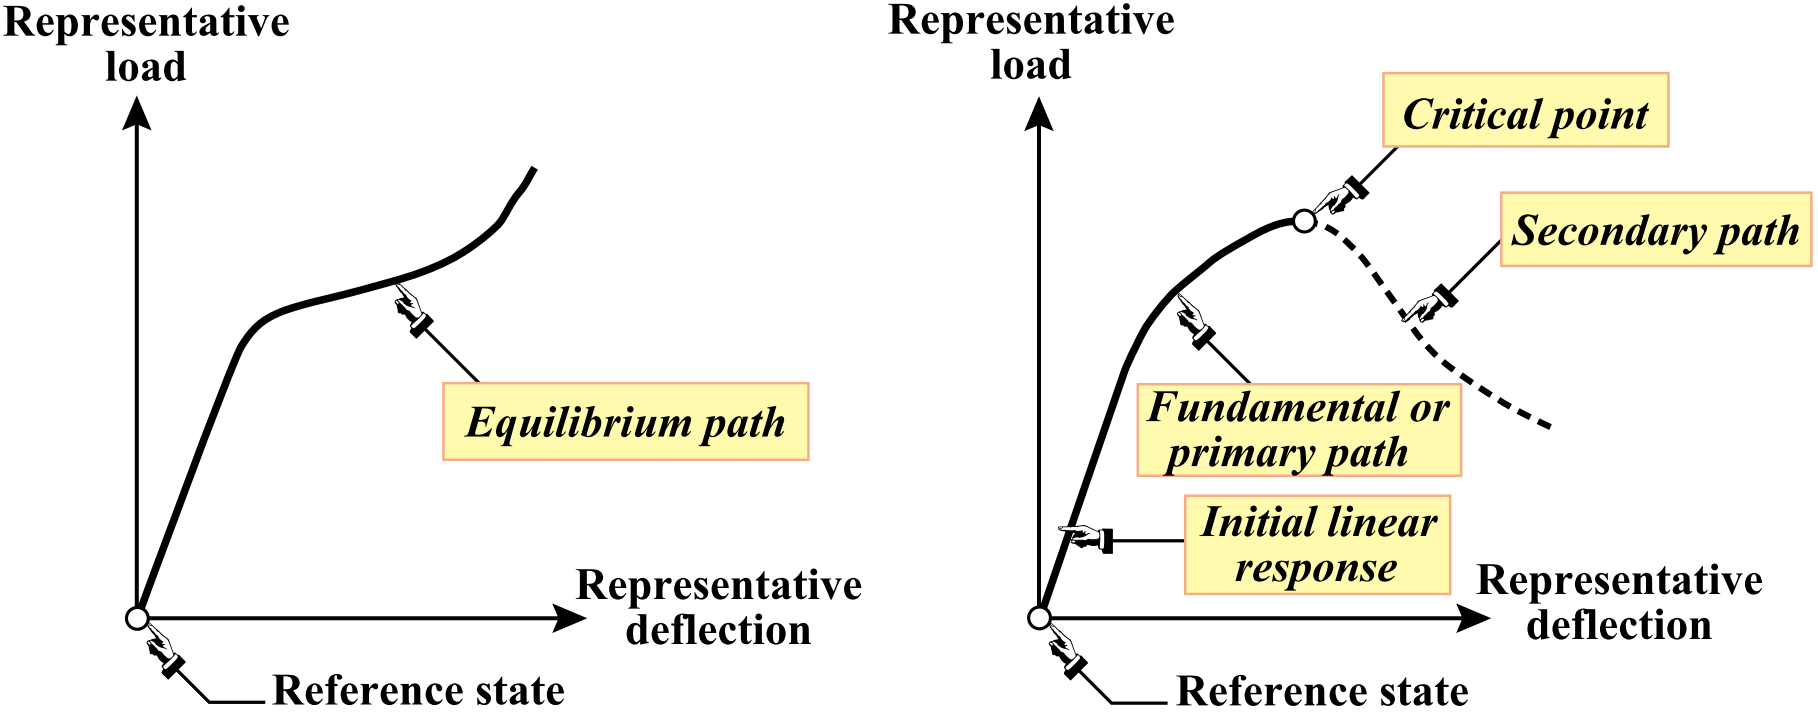
\includegraphics[width=12cm]{images/stability_response_diagram.png}
	\caption{Examples of response diagrams \cite{FelippaNFEMTour2016}}
	\label{stab0}
\end{figure}

The equilibrium path of a response diagram unsurprisingly indicates the points in load-deflection space where the structure is in equilibrium, that is, the residual vector $\mathbf{r}$ of the system vanishes. If the scope of structures considered is limited to static linear elastic structures subject to conservative loading characterised by a load factor $\lambda$ linearly scaling the external load vector $\mathbf{f}$, the residual itself is defined as the gradient of the structure's energy $\Pi$ \cite{FelippaNFEMCrit2016}:

\begin{equation}
\mathbf{r}(\mathbf{u},\lambda) = \frac{\partial \Pi (\mathbf{u},\lambda)}{\partial \mathbf{u}}
\label{eqstab0}
\end{equation}

The tangent stiffness matrix of the system is intuitively the slope of the equilibrium path, or, more precisely, the Hessian of the structure's energy:

\begin{equation} 
\mathbf{K} = 
\frac{\partial \mathbf{r} (\mathbf{u},\lambda)}{\partial \mathbf{u}} = 
\frac{\partial^2 \Pi (\mathbf{u},\lambda)}{\partial \mathbf{u}\partial \mathbf{u}}
\label{eqstab01}
\end{equation}

Recalling that the equilibrium path of a structure is defined by a vanishing residual, it can be presented in a variety of forms:

\begin{equation} 
\mathbf{r}(\mathbf{u},\lambda) = 
\frac{\partial \Pi (\mathbf{u},\lambda)}{\partial \mathbf{u}} =
\mathbf{K}(\mathbf{u},\lambda) \mathbf{u} - \mathbf{f}(\mathbf{u},\lambda) =
0
\label{eqstab02}
\end{equation}

The above expansion offers a variety of perspectives in which to interpret the equilibrium path. A nod to virtual work methods via variation of system energy is present as well as a simple re-arrangement of the well known $\mathbf{Ku} = \mathbf{f}$ introduced in Bachelor FEM courses.

\section{Stability criterion}
 If the aforementioned Euler beam buckling example is fully examined (refer Appendix XXX), it is apparent that the well known Euler critical load formula precipitates by setting the determinant of the system stiffness matrix to zero. In general, loss of structural stability only occurs at critical points $(\mathbf{u}_c,\lambda_c)$ where the determinant of the tangent stiffness matrix vanishes:
 
 \begin{equation} 
 det\big[\mathbf{K}(\mathbf{u}_c,\lambda_c)\big] = 0
 \label{eqstab1}
 \end{equation}
 
 In this Euler case, the instability is manifested by way of bifurcation, commonly referred to as buckling. Bifurcation points designate a critical point in the load-displacement space of the structure where two or more equilibrium paths meet. At these points structure may unpredictably switch equilibrium paths physically manifesting itself as dramatic large deflections. Indeed, in the buckling of a circular-sectioned beam, the direction of buckling deformation is entirely unpredictable (bar coaxing imperfections) with many equilibrium paths coincident at the bifurcation point. Limit, or snap-through, points are the other type of instability that may occur at critical points. In this regime, the critical point coincides with a minimum, maximum or inflection of the load parameter $\lambda$. For an everyday example of snap-through, one can consider an umbrella suddenly inverting in a strong storm, demonstrating that once the snapping wind load is reached predictably large deformations are subsequently observed. The following figure \ref{stab1}(a) illustrates the nature of both instability types on a load-deflection diagram.

\begin{figure}[H]
	\subfloat[Critical points of a response diagram]
	{\label{ref_label2}
		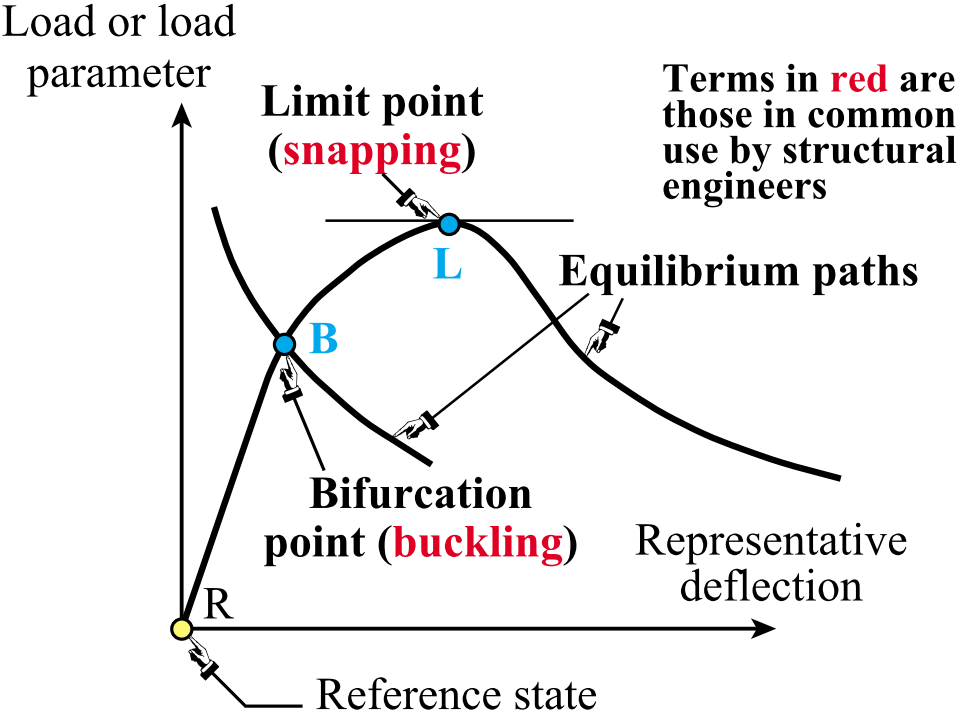
\includegraphics[width=7.3cm]
		{images/stability_eq_path.png}}
	\subfloat[Bifurcation-driven structure critical load]
	{\label{ref_label2}
		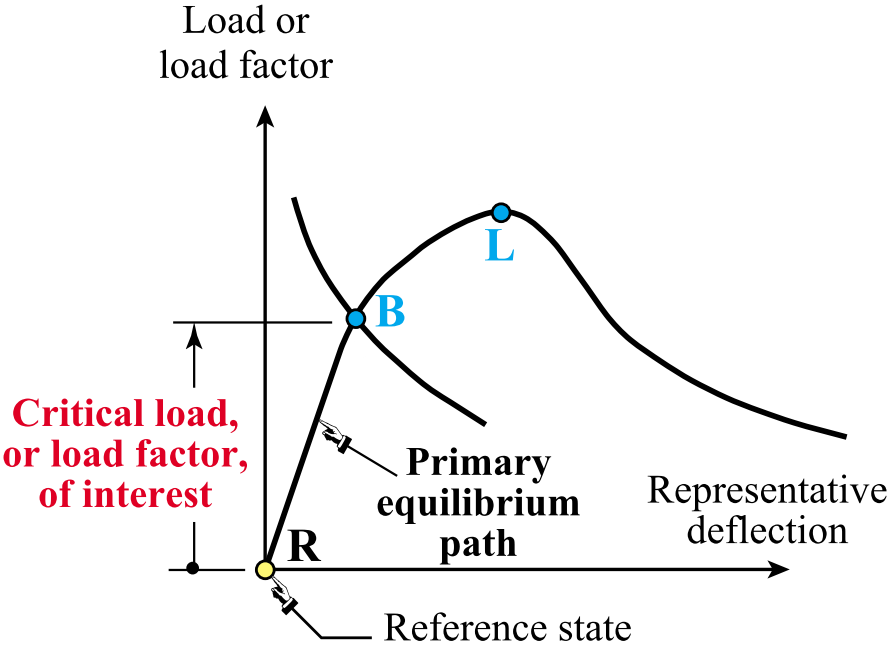
\includegraphics[width=7.3cm]
		{images/stability_buckling.png}}
	\caption{\label{stab1}Stability analysis response diagrams \cite{FelippaStabilityBasics2016}}
\end{figure}

It's clear that after both critical points, as depicted in figure \ref{stab1}(a), the structure looses a significant proportion of it's stiffness indicated by the reduced load required for continual increases of deflection. In this post-buckling state the original function, and indeed safety, of the structure (for example, a roof or building) is likely to be significantly compromised. If such a structural critical point exists at a load level less than the design load cases considered for allowable deflections and stresses then the structure cannot be regarded as properly engineered. Figure \ref{stab1}(b) indicates the critical stability load of the structure, which is the load corresponding to the first critical point on the response diagram. Another more stringent approach is to determine the lowest load factor throughout the whole equilibrium path, including the post-critical regime, and take this as the critical stability load.

Despite the need for stability analysis to be regularly considered throughout engineering design, the effort and level of analysis required is clearly quite significant for even simple systems. As such, a linearised approach termed Linear prebuckling analysis, is often employed.

\section{Linear prebuckling analysis}
Linear prebuckling (LPB) analysis offers a reduced insight into the stability characteristics of the structure at a fraction of the computational expense required for a full non-linear equilibrium path analysis.

In order to further interrogate the nature of structural stability, and how it may be simplified, the tangent stiffness matrix in equation \ref{eqstab1} can be decomposed. The total tangent matrix is made up of the material stiffness matrix $\mathbf{K}_m$ (itself composed of the elastic stiffness $\mathbf{K}_e$ and initial displacement stiffness $\mathbf{K}_u$) and the geometric stiffness matrix $\mathbf{K}_g$. Thus equation \ref{eqstab1} can be expanded accordingly:

\begin{equation} 
det\big[
\mathbf{K}_e +
\mathbf{K}_u(\mathbf{u}_0) +
\mathbf{K}_g(\mathbf{u}_c,\lambda_c)
\big] = 
det\big[
\mathbf{K}_m +
\mathbf{K}_g(\mathbf{u}_c,\lambda_c)
\big] = 0
\label{eqstab2}
\end{equation}

It's apparent the expression can be characterized as an eigenvalue problem, thus the eigenvector $\mathbf{z} \neq \mathbf{0}$ corresponding to bifurcation mode shapes can be introduced:

\begin{equation} 
det\big[
\mathbf{K}_m +
\mathbf{K}_g(\mathbf{u}_c,\lambda_c)
\big]\mathbf{z} = 0
\label{eqstab3}
\end{equation}

The non-linear eigenvalue problem can be presented in a linearised form:

\begin{equation} 
det\big[
\mathbf{K}_m +
\hat{\lambda}
\mathbf{K}_g(\mathbf{u}_i,\lambda_i)
\big]\mathbf{z} = 0
\label{eqstab4}
\end{equation}

Equations \ref{eqstab3} and \ref{eqstab4} are identical if $\hat{\lambda}
 = 1,\ \lambda_i = \lambda_c$ and $u_i = u_c$.
 
 If the structure under analysis is considered suitably stiff, with infinitesimal displacements $\mathbf{u} \approx 0$ in the pre-buckling regime and negligible effects of initial displacements ($\mathbf{K}_u(\mathbf{u} \approx 0) \approx 0$), then a simplified stability eigen-problem can be presented:
 
 \begin{equation} 
 det\big[
 \mathbf{K}_e +
{\lambda}
 \mathbf{K}_g(\lambda_{ref})
 \big]\mathbf{z} = 0
 \label{eqstab5}
 \end{equation}
 
 The LPB equation above relies on the additional assumptions that the structure remains linearly elastic until buckling and the structure and loading have no imperfections \cite{FelippaStabilityBasics2016}. It's also clear that the geometric stiffness matrix is assumed to scale proportionally with the load factor, which further relies on the assumption of a linearly elastic structure. Along with these assumptions, LPB carries some important limitations. The first of which is the typical over-estimation of the true buckling limit, with the accuracy deteriorating as the pre-buckling structural behaviour becomes more non-linear. The second limitation is the inability to distinguish between bifurcation and limit points, with all critical points transformed into bifurcation points. A consequence of this is that the recovered eigenvector associated with a limit point reported as a bifurcation point will be erroneous.
 
 Despite the large swathe of assumptions and limitations accompanying LPB, it is no doubt a sensible and computationally-efficient approach when applied to suitably stiff linear elastic structures, which indeed form the bulk of industrial engineering structures.

\section{Stability analysis example}

To illustrate the various aspects stability analysis, including response diagrams and the comparison of non-linear and linear critical point analysis, an example two truss system is considered. The full analysis can be found in Appendix XXXX, with only key results reproduced below.

\begin{figure}[H]
	\centering
	\def\svgwidth{\columnwidth}
	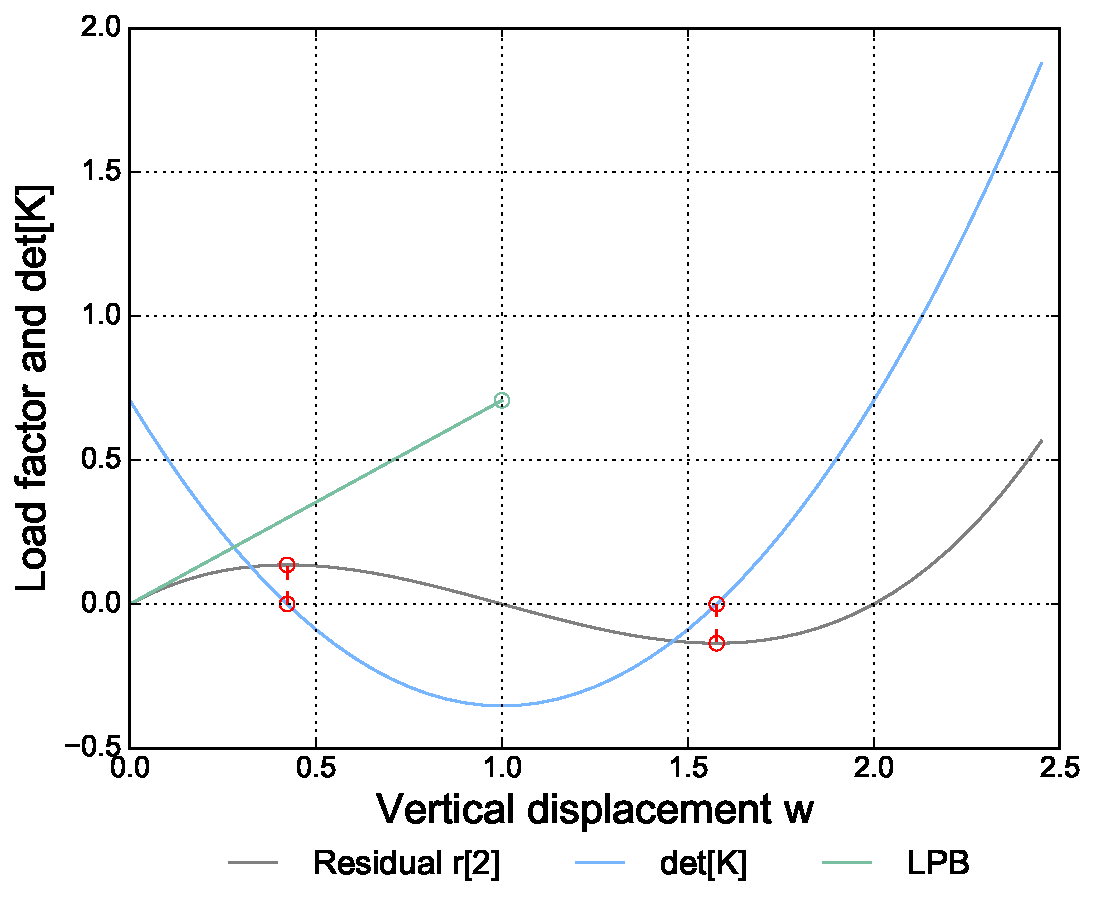
\includegraphics[width=12cm]{images/stability_analysis_mises_truss_1x1.pdf}
	\caption{Response diagram of Mises truss}
	\label{stab2}
\end{figure}

asdfasdf

\begin{figure}[H]
	\centering
	\def\svgwidth{\columnwidth}
	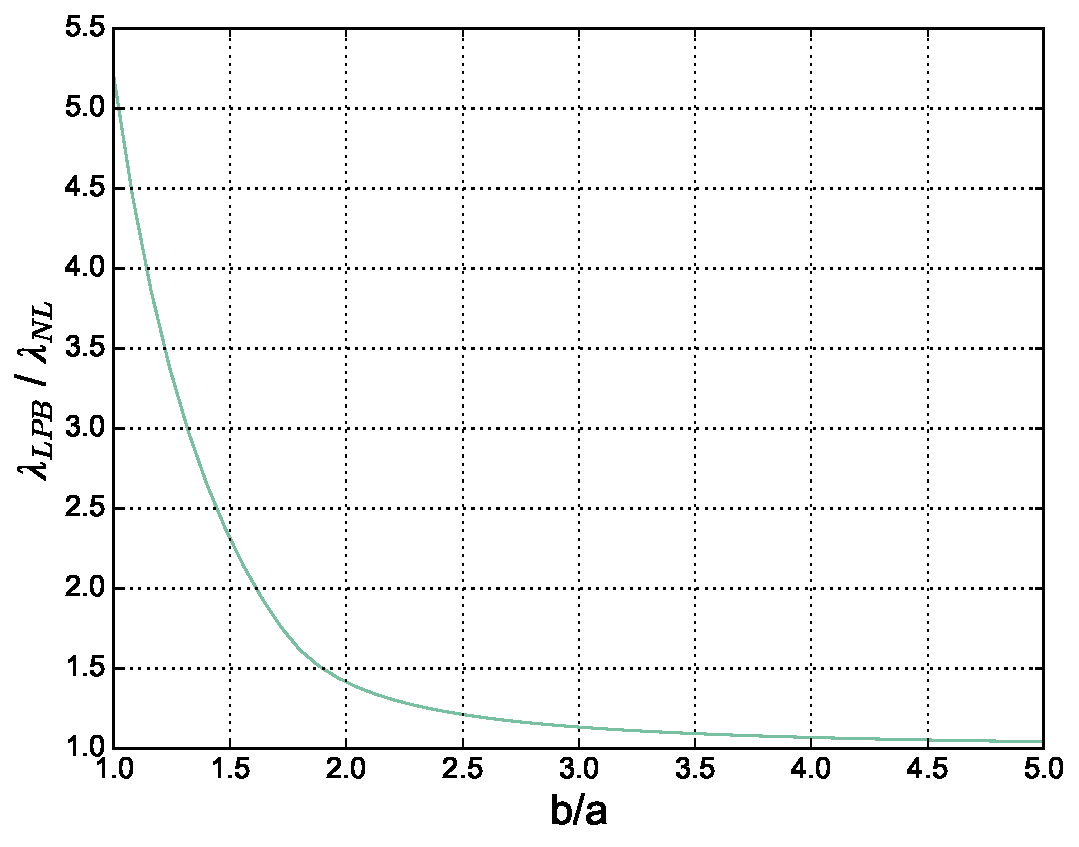
\includegraphics[width=12cm]{images/stability_analysis_mises_truss_lpb.pdf}
	\caption{Ratio of Mises truss LPB and NL critical load factors across varying geometry}
	\label{stab3}
\end{figure}


- Definition

- Examples of where it's important. P-delta effect

- Critical points, det = 0

- Example, just show summary, put full calc in appendix

- Linear prebuckling definiton

- Linear pre-buckling example

- Implementation of LPB